\chapter{Complete search}

\key{Complete search}
is a general method that can be used
to solve almost any algorithm problem.
The idea is to generate all possible
solutions to the problem using brute force,
and then select the best solution or count the
number of solutions, depending on the problem.

Complete search is a good technique
if there is enough time to go through all the solutions,
because the search is usually easy to implement
and it always gives the correct answer.
If complete search is too slow,
other techniques, such as greedy algorithms or
dynamic programming, may be needed.

\section{Generating subsets}

\index{subset}

We first consider the problem of generating
all subsets of a set of $n$ elements.
There are two common methods for this:
we can either implement a recursive search
or use bit operations of integers.

\subsubsection{Method 1}

An elegant way to go through all subsets
of a set is to use recursion.
The following function
generates the subsets of the set
$\{1,2,\ldots,n\}$.
The function maintains a vector
that will contain the elements of each subset.
The search begins when the function is called
with parameter 1.

\begin{lstlisting}
void gen(int k) {
    if (k == n+1) {
        // process subset v
    } else {
        gen(k+1);
        v.push_back(k);
        gen(k+1);
        v.pop_back();
    }
}
\end{lstlisting}

The parameter $k$ is the next
candidate to be included in the subset.
The function considers two cases that both
generate a recursive call:
either $k$ is included or not included in the subset.
Finally, when $k=n+1$, all elements have been processed
and one subset has been generated.

The following tree illustrates how the function is
called when $n=3$.
We can always choose either the left branch
($k$ is not included in the subset) or the right branch
($k$ is included in the subset).

\begin{center}
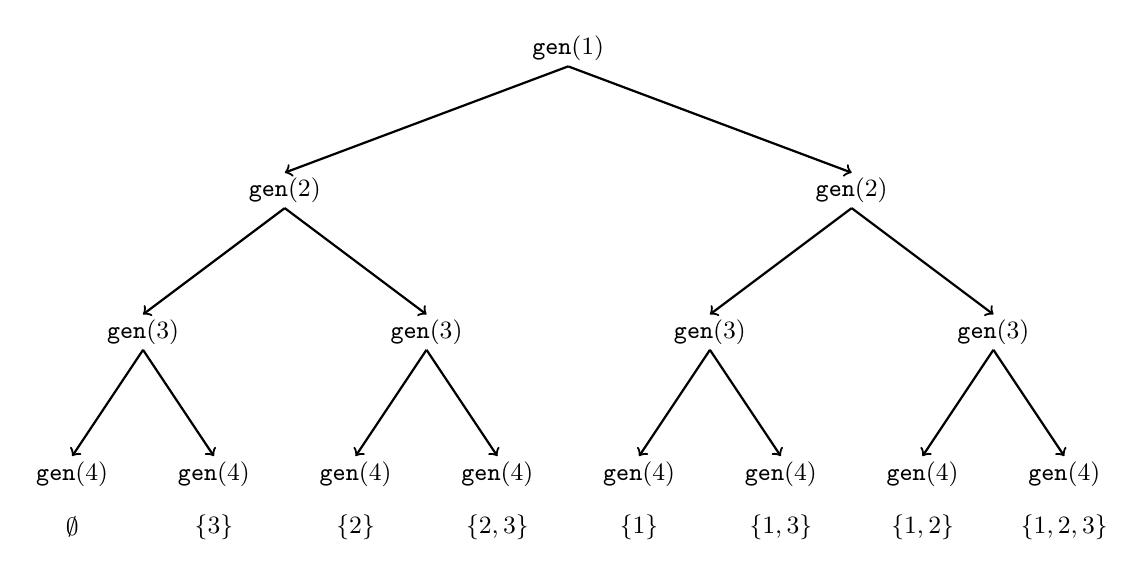
\begin{tikzpicture}[scale=.45]
  \begin{scope}
    \small
    \node at (0,0) {$\texttt{gen}(1)$};

    \node at (-8,-4) {$\texttt{gen}(2)$};
    \node at (8,-4) {$\texttt{gen}(2)$};

    \path[draw,thick,->] (0,0-0.5) -- (-8,-4+0.5);
    \path[draw,thick,->] (0,0-0.5) -- (8,-4+0.5);

    \node at (-12,-8) {$\texttt{gen}(3)$};
    \node at (-4,-8) {$\texttt{gen}(3)$};
    \node at (4,-8) {$\texttt{gen}(3)$};
    \node at (12,-8) {$\texttt{gen}(3)$};

    \path[draw,thick,->] (-8,-4-0.5) -- (-12,-8+0.5);
    \path[draw,thick,->] (-8,-4-0.5) -- (-4,-8+0.5);
    \path[draw,thick,->] (8,-4-0.5) -- (4,-8+0.5);
    \path[draw,thick,->] (8,-4-0.5) -- (12,-8+0.5);

    \node at (-14,-12) {$\texttt{gen}(4)$};
    \node at (-10,-12) {$\texttt{gen}(4)$};
    \node at (-6,-12) {$\texttt{gen}(4)$};
    \node at (-2,-12) {$\texttt{gen}(4)$};
    \node at (2,-12) {$\texttt{gen}(4)$};
    \node at (6,-12) {$\texttt{gen}(4)$};
    \node at (10,-12) {$\texttt{gen}(4)$};
    \node at (14,-12) {$\texttt{gen}(4)$};

    \node at (-14,-13.5) {$\emptyset$};
    \node at (-10,-13.5) {$\{3\}$};
    \node at (-6,-13.5) {$\{2\}$};
    \node at (-2,-13.5) {$\{2,3\}$};
    \node at (2,-13.5) {$\{1\}$};
    \node at (6,-13.5) {$\{1,3\}$};
    \node at (10,-13.5) {$\{1,2\}$};
    \node at (14,-13.5) {$\{1,2,3\}$};


    \path[draw,thick,->] (-12,-8-0.5) -- (-14,-12+0.5);
    \path[draw,thick,->] (-12,-8-0.5) -- (-10,-12+0.5);
    \path[draw,thick,->] (-4,-8-0.5) -- (-6,-12+0.5);
    \path[draw,thick,->] (-4,-8-0.5) -- (-2,-12+0.5);
    \path[draw,thick,->] (4,-8-0.5) -- (2,-12+0.5);
    \path[draw,thick,->] (4,-8-0.5) -- (6,-12+0.5);
    \path[draw,thick,->] (12,-8-0.5) -- (10,-12+0.5);
    \path[draw,thick,->] (12,-8-0.5) -- (14,-12+0.5);
\end{scope}
\end{tikzpicture}
\end{center}

\subsubsection{Method 2}

Another way to generate subsets is to exploit
the bit representation of integers.
Each subset of a set of $n$ elements
can be represented as a sequence of $n$ bits,
which corresponds to an integer between $0 \ldots 2^n-1$.
The ones in the bit sequence indicate
which elements are included in the subset.

The usual convention is that the $k$th element
is included in the subset exactly when the $k$th last bit
in the sequence is one.
For example, the bit representation of 25
is 11001, that corresponds to the subset $\{1,4,5\}$.

The following code goes through all subsets
of a set of $n$ elements

\begin{lstlisting}
for (int b = 0; b < (1<<n); b++) {
    // process subset b
}
\end{lstlisting}

The following code shows how we can find
the elements of a subset that corresponds to a bit sequence.
When processing each subset,
the code builds a vector that contains the
elements in the subset.

\begin{lstlisting}
for (int b = 0; b < (1<<n); b++) {
    vector<int> v;
    for (int i = 0; i < n; i++) {
        if (b&(1<<i)) v.push_back(i+1);
    }
}
\end{lstlisting}

\section{Generating permutations}

\index{permutation}

Next we will consider the problem of generating
all permutations of a set of $n$ elements.
Again, there are two approaches:
we can either use recursion or go through the
permutations iteratively.

\subsubsection{Method 1}

Like subsets, permutations can be generated
using recursion.
The following function goes
through the permutations of the set $\{1,2,\ldots,n\}$.
The function builds a vector that contains
the elements in the permutation,
and the search begins when the function is
called without parameters.

\begin{lstlisting}
void gen() {
    if (v.size() == n) {
        // process permutation v
    } else {
        for (int i = 1; i <= n; i++) {
            if (p[i]) continue;
            p[i] = 1;
            v.push_back(i);
            gen();
            p[i] = 0;
            v.pop_back();
        }
    }
}
\end{lstlisting}

Each function call adds a new element to
the vector \texttt{v}.
The array \texttt{p} indicates which
elements are already included in the permutation:
if $\texttt{p}[k]=0$, element $k$ is not included,
and if $\texttt{p}[k]=1$, element $k$ is included.
If the size of \texttt{v} equals the size of the set,
a permutation has been generated.

\subsubsection{Method 2}

\index{next\_permutation@\texttt{next\_permutation}}

Another method for generating permutations
is to begin with the permutation
$\{1,2,\ldots,n\}$ and repeatedly
use a function that constructs the next permutation
in increasing order.
The C++ standard library contains the function
\texttt{next\_permutation} that can be used for this:

\begin{lstlisting}
vector<int> v;
for (int i = 1; i <= n; i++) {
    v.push_back(i);
}
do {
    // process permutation v
} while (next_permutation(v.begin(),v.end()));
\end{lstlisting}

\section{Backtracking}

\index{backtracking}

A \key{backtracking} algorithm
begins with an empty solution
and extends the solution step by step.
The search recursively
goes through all different ways how
a solution can be constructed.

\index{queen problem}

As an example, consider the \key{queen problem}
where the task is to calculate the number
of ways we can place $n$ queens to
an $n \times n$ chessboard so that
no two queens attack each other.
For example, when $n=4$,
there are two possible solutions to the problem:

\begin{center}
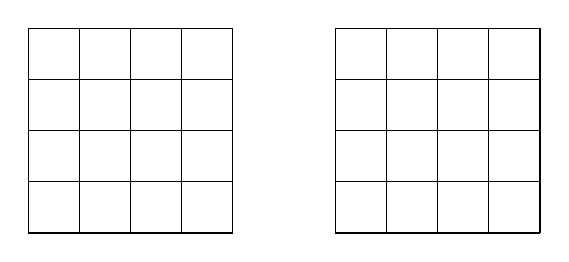
\begin{tikzpicture}[scale=.65]
  \begin{scope}
    \draw (0, 0) grid (4, 4);
    \node at (1.5,3.5) {\symqueen};
    \node at (3.5,2.5) {\symqueen};
    \node at (0.5,1.5) {\symqueen};
    \node at (2.5,0.5) {\symqueen};

    \draw (6, 0) grid (10, 4);
    \node at (6+2.5,3.5) {\symqueen};
    \node at (6+0.5,2.5) {\symqueen};
    \node at (6+3.5,1.5) {\symqueen};
    \node at (6+1.5,0.5) {\symqueen};

  \end{scope}
\end{tikzpicture}
\end{center}

The problem can be solved using backtracking
by placing queens to the board row by row.
More precisely, exactly one queen will
be placed to each row so that no queen attacks
any of the queens placed before.
A solution has been found when all
$n$ queens have been placed to the board.

For example, when $n=4$,
some partial solutions generated by
the backtracking algorithm are as follows:

\begin{center}
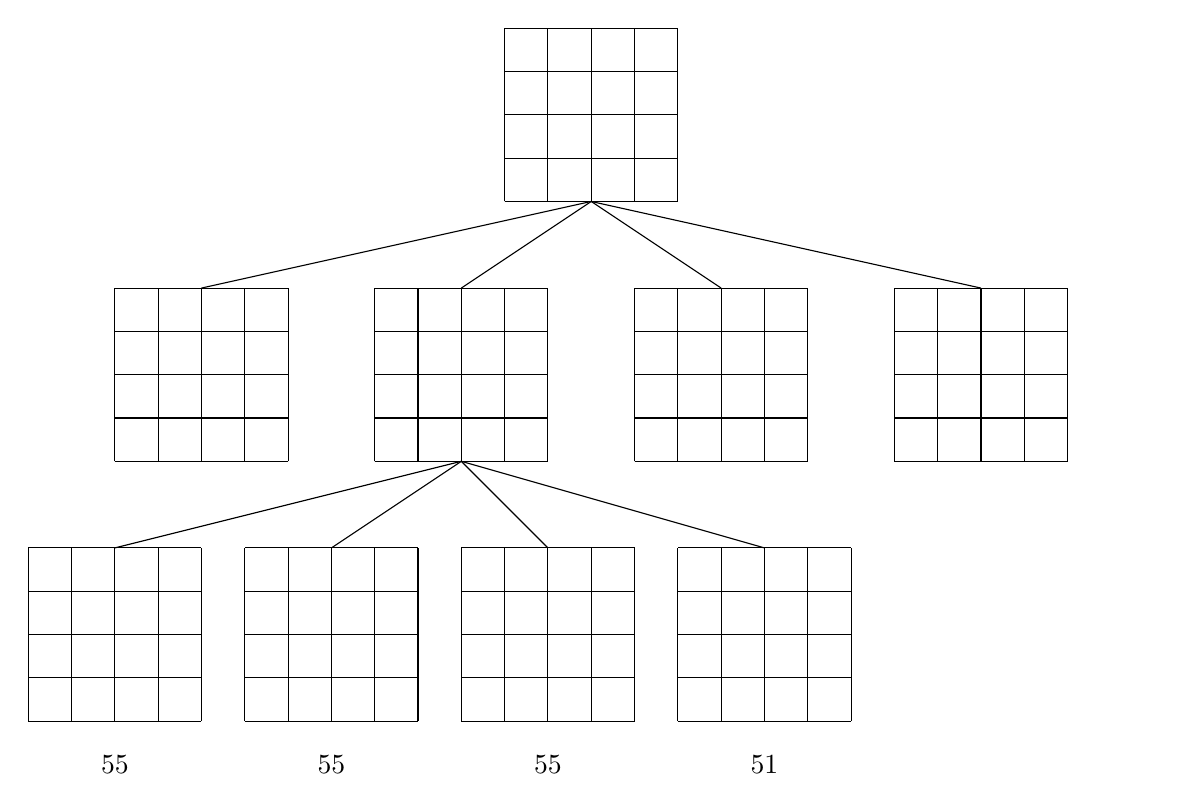
\begin{tikzpicture}[scale=.55]
  \begin{scope}
    \draw (0, 0) grid (4, 4);

    \draw (-9, -6) grid (-5, -2);
    \draw (-3, -6) grid (1, -2);
    \draw (3, -6) grid (7, -2);
    \draw (9, -6) grid (13, -2);

    \node at (-9+0.5,-3+0.5) {\symqueen};
    \node at (-3+1+0.5,-3+0.5) {\symqueen};
    \node at (3+2+0.5,-3+0.5) {\symqueen};
    \node at (9+3+0.5,-3+0.5) {\symqueen};

    \draw (2,0) -- (-7,-2);
    \draw (2,0) -- (-1,-2);
    \draw (2,0) -- (5,-2);
    \draw (2,0) -- (11,-2);

    \draw (-11, -12) grid (-7, -8);
    \draw (-6, -12) grid (-2, -8);
    \draw (-1, -12) grid (3, -8);
    \draw (4, -12) grid (8, -8);
    \draw[white] (11, -12) grid (15, -8);
    \node at (-11+1+0.5,-9+0.5) {\symqueen};
    \node at (-6+1+0.5,-9+0.5) {\symqueen};
    \node at (-1+1+0.5,-9+0.5) {\symqueen};
    \node at (4+1+0.5,-9+0.5) {\symqueen};
    \node at (-11+0+0.5,-10+0.5) {\symqueen};
    \node at (-6+1+0.5,-10+0.5) {\symqueen};
    \node at (-1+2+0.5,-10+0.5) {\symqueen};
    \node at (4+3+0.5,-10+0.5) {\symqueen};

    \draw (-1,-6) -- (-9,-8);
    \draw (-1,-6) -- (-4,-8);
    \draw (-1,-6) -- (1,-8);
    \draw (-1,-6) -- (6,-8);

    \node at (-9,-13) {\ding{55}};
    \node at (-4,-13) {\ding{55}};
    \node at (1,-13) {\ding{55}};
    \node at (6,-13) {\ding{51}};

  \end{scope}
\end{tikzpicture}
\end{center}

At the bottom level, the three first boards
are not valid, because the queens attack each other.
However, the fourth board is valid
and it can be extended to a complete solution by
placing two more queens to the board.

\begin{samepage}
The following code implements the search:
\begin{lstlisting}
void search(int y) {
    if (y == n) {
        c++;
        return;
    }
    for (int x = 0; x < n; x++) {
        if (r1[x] || r2[x+y] || r3[x-y+n-1]) continue;
        r1[x] = r2[x+y] = r3[x-y+n-1] = 1;
        search(y+1);
        r1[x] = r2[x+y] = r3[x-y+n-1] = 0;
    }
}
\end{lstlisting}
\end{samepage}
The search begins by calling \texttt{search(0)}.
The size of the board is in the variable $n$,
and the code calculates the number of solutions
to the variable $c$.

The code assumes that the rows and columns
of the board are numbered from 0.
The function places a queen to row $y$
where $0 \le y < n$.
Finally, if $y=n$, a solution has been found
and the variable $c$ is increased by one.

The array \texttt{r1} keeps track of the columns
that already contain a queen,
and the arrays \texttt{r2} and \texttt{r3}
keep track of the diagonals.
It is not allowed to add another queen to a
column or diagonal that already contains a queen. 
For example, the rows and diagonals of
the $4 \times 4$ board are numbered as follows:

\begin{center}
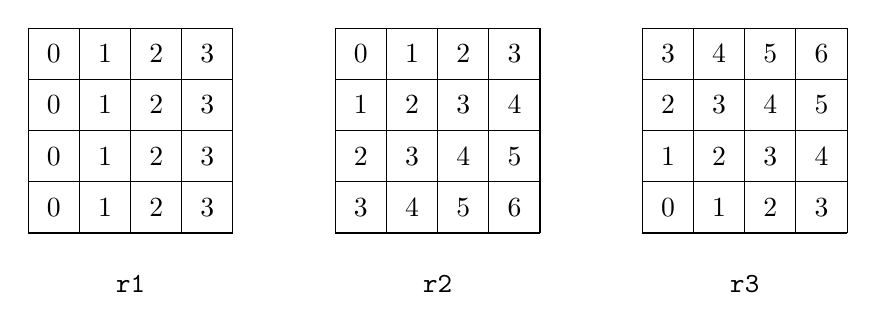
\begin{tikzpicture}[scale=.65]
  \begin{scope}
    \draw (0-6, 0) grid (4-6, 4);
    \node at (-6+0.5,3.5) {$0$};
    \node at (-6+1.5,3.5) {$1$};
    \node at (-6+2.5,3.5) {$2$};
    \node at (-6+3.5,3.5) {$3$};
    \node at (-6+0.5,2.5) {$0$};
    \node at (-6+1.5,2.5) {$1$};
    \node at (-6+2.5,2.5) {$2$};
    \node at (-6+3.5,2.5) {$3$};
    \node at (-6+0.5,1.5) {$0$};
    \node at (-6+1.5,1.5) {$1$};
    \node at (-6+2.5,1.5) {$2$};
    \node at (-6+3.5,1.5) {$3$};
    \node at (-6+0.5,0.5) {$0$};
    \node at (-6+1.5,0.5) {$1$};
    \node at (-6+2.5,0.5) {$2$};
    \node at (-6+3.5,0.5) {$3$};

    \draw (0, 0) grid (4, 4);
    \node at (0.5,3.5) {$0$};
    \node at (1.5,3.5) {$1$};
    \node at (2.5,3.5) {$2$};
    \node at (3.5,3.5) {$3$};
    \node at (0.5,2.5) {$1$};
    \node at (1.5,2.5) {$2$};
    \node at (2.5,2.5) {$3$};
    \node at (3.5,2.5) {$4$};
    \node at (0.5,1.5) {$2$};
    \node at (1.5,1.5) {$3$};
    \node at (2.5,1.5) {$4$};
    \node at (3.5,1.5) {$5$};
    \node at (0.5,0.5) {$3$};
    \node at (1.5,0.5) {$4$};
    \node at (2.5,0.5) {$5$};
    \node at (3.5,0.5) {$6$};

    \draw (6, 0) grid (10, 4);
    \node at (6.5,3.5) {$3$};
    \node at (7.5,3.5) {$4$};
    \node at (8.5,3.5) {$5$};
    \node at (9.5,3.5) {$6$};
    \node at (6.5,2.5) {$2$};
    \node at (7.5,2.5) {$3$};
    \node at (8.5,2.5) {$4$};
    \node at (9.5,2.5) {$5$};
    \node at (6.5,1.5) {$1$};
    \node at (7.5,1.5) {$2$};
    \node at (8.5,1.5) {$3$};
    \node at (9.5,1.5) {$4$};
    \node at (6.5,0.5) {$0$};
    \node at (7.5,0.5) {$1$};
    \node at (8.5,0.5) {$2$};
    \node at (9.5,0.5) {$3$};

    \node at (-4,-1) {\texttt{r1}};
    \node at (2,-1) {\texttt{r2}};
    \node at (8,-1) {\texttt{r3}};

  \end{scope}
\end{tikzpicture}
\end{center}

The above backtracking
algorithm tells us that
there are 92 ways to place 8
queens to the $8 \times 8$ chessboard.
When $n$ increases, the search quickly becomes slow,
because the number of the solutions increases
exponentially.
For example, calculating the ways to
place 16 queens to the $16 \times 16$
chessboard already takes about a minute
on a modern computer
(there are 14772512 solutions).

\section{Pruning the search}

We can often optimize backtracking
by pruning the search tree.
The idea is to add ''intelligence'' to the algorithm
so that it will notice as soon as possible
if a partial solution cannot be extended
to a complete solution.
Such optimizations can have a tremendous
effect on the efficiency of the search.

Let us consider a problem
of calculating the number of paths
in an $n \times n$ grid from the upper-left corner
to the lower-right corner so that each square
will be visited exactly once.
For example, in a $7 \times 7$ grid,
there are 111712 such paths.
One of the paths is as follows:

\begin{center}
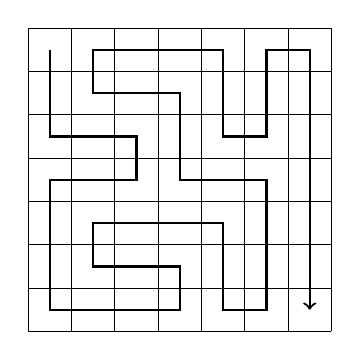
\begin{tikzpicture}[scale=.55]
  \begin{scope}
    \draw (0, 0) grid (7, 7);
    \draw[thick,->] (0.5,6.5) -- (0.5,4.5) -- (2.5,4.5) --
          (2.5,3.5) -- (0.5,3.5) -- (0.5,0.5) --
          (3.5,0.5) -- (3.5,1.5) -- (1.5,1.5) --
          (1.5,2.5) -- (4.5,2.5) -- (4.5,0.5) --
          (5.5,0.5) -- (5.5,3.5) -- (3.5,3.5) --
          (3.5,5.5) -- (1.5,5.5) -- (1.5,6.5) --
          (4.5,6.5) -- (4.5,4.5) -- (5.5,4.5) --
          (5.5,6.5) -- (6.5,6.5) -- (6.5,0.5);
  \end{scope}
\end{tikzpicture}
\end{center}

We will concentrate on the $7 \times 7$ case,
because its level of difficulty is appropriate to our needs.
We begin with a straightforward backtracking algorithm,
and then optimize it step by step using observations
how the search can be pruned.
After each optimization, we measure the running time
of the algorithm and the number of recursive calls,
so that we will clearly see the effect of each
optimization on the efficiency of the search.

\subsubsection{Basic algorithm}

The first version of the algorithm does not contain
any optimizations. We simply use backtracking to generate
all possible paths from the upper-left corner to
the lower-right corner and count the number of such paths.

\begin{itemize}
\item
running time: 483 seconds
\item
recursive calls: 76 billions
\end{itemize}

\subsubsection{Optimization 1}

In any solution, we first move one step
down or right.
There are always two paths that 
are symmetric
about the diagonal of the grid
after the first step.
For example, the following paths are symmetric:

\begin{center}
\begin{tabular}{ccc}
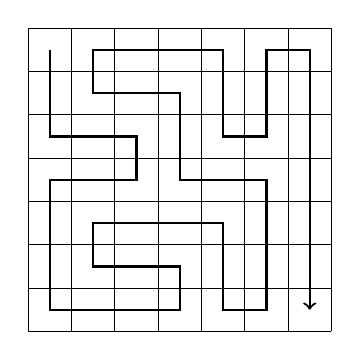
\begin{tikzpicture}[scale=.55]
  \begin{scope}
    \draw (0, 0) grid (7, 7);
    \draw[thick,->] (0.5,6.5) -- (0.5,4.5) -- (2.5,4.5) --
          (2.5,3.5) -- (0.5,3.5) -- (0.5,0.5) --
          (3.5,0.5) -- (3.5,1.5) -- (1.5,1.5) --
          (1.5,2.5) -- (4.5,2.5) -- (4.5,0.5) --
          (5.5,0.5) -- (5.5,3.5) -- (3.5,3.5) --
          (3.5,5.5) -- (1.5,5.5) -- (1.5,6.5) --
          (4.5,6.5) -- (4.5,4.5) -- (5.5,4.5) --
          (5.5,6.5) -- (6.5,6.5) -- (6.5,0.5);
  \end{scope}
\end{tikzpicture}
& \hspace{20px}
& 
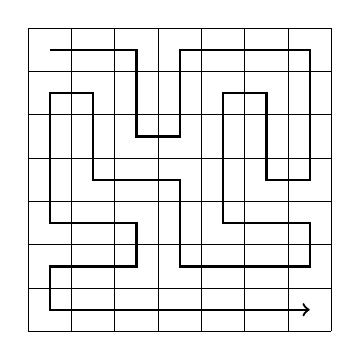
\begin{tikzpicture}[scale=.55]
  \begin{scope}[yscale=1,xscale=-1,rotate=-90]
    \draw (0, 0) grid (7, 7);
    \draw[thick,->] (0.5,6.5) -- (0.5,4.5) -- (2.5,4.5) --
          (2.5,3.5) -- (0.5,3.5) -- (0.5,0.5) --
          (3.5,0.5) -- (3.5,1.5) -- (1.5,1.5) --
          (1.5,2.5) -- (4.5,2.5) -- (4.5,0.5) --
          (5.5,0.5) -- (5.5,3.5) -- (3.5,3.5) --
          (3.5,5.5) -- (1.5,5.5) -- (1.5,6.5) --
          (4.5,6.5) -- (4.5,4.5) -- (5.5,4.5) --
          (5.5,6.5) -- (6.5,6.5) -- (6.5,0.5);
  \end{scope}
\end{tikzpicture}
\end{tabular}
\end{center}

Hence, we can decide that we always first
move one step down,
and finally multiply the number of the solutions by two.

\begin{itemize}
\item
running time: 244 seconds
\item
recursive calls: 38 billions
\end{itemize}

\subsubsection{Optimization 2}

If the path reaches the lower-right square
before it has visited all other squares of the grid,
it is clear that
it will not be possible to complete the solution.
An example of this is the following path:

\begin{center}
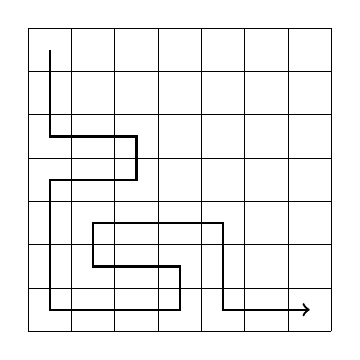
\begin{tikzpicture}[scale=.55]
  \begin{scope}
    \draw (0, 0) grid (7, 7);
    \draw[thick,->] (0.5,6.5) -- (0.5,4.5) -- (2.5,4.5) --
          (2.5,3.5) -- (0.5,3.5) -- (0.5,0.5) --
          (3.5,0.5) -- (3.5,1.5) -- (1.5,1.5) --
          (1.5,2.5) -- (4.5,2.5) -- (4.5,0.5) --
          (6.5,0.5);
  \end{scope}
\end{tikzpicture}
\end{center}
Using this observation, we can terminate the search
immediately if we reach the lower-right square too early.
\begin{itemize}
\item
running time: 119 seconds
\item
recursive calls: 20 billions
\end{itemize}

\subsubsection{Optimization 3}

If the path touches the wall so that there is
an unvisited square on both sides,
the grid splits into two parts.
For example, in the following path
both the left and right squares
are unvisited:

\begin{center}
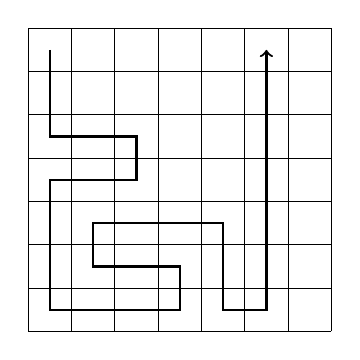
\begin{tikzpicture}[scale=.55]
  \begin{scope}
    \draw (0, 0) grid (7, 7);
    \draw[thick,->] (0.5,6.5) -- (0.5,4.5) -- (2.5,4.5) --
          (2.5,3.5) -- (0.5,3.5) -- (0.5,0.5) --
          (3.5,0.5) -- (3.5,1.5) -- (1.5,1.5) --
          (1.5,2.5) -- (4.5,2.5) -- (4.5,0.5) --
          (5.5,0.5) -- (5.5,6.5);
  \end{scope}
\end{tikzpicture}
\end{center}
Now it will not be possible to visit every square,
so we can terminate the search.
It turns out that this optimization is very useful:

\begin{itemize}
\item
running time: 1.8 seconds
\item
recursive calls: 221 millions
\end{itemize}

\subsubsection{Optimization 4}

The idea of the previous optimization
can be generalized:
the grid splits into two parts
if the top and bottom neighbors
of the current square are unvisited and
the left and right neighbors are
wall or visited (or vice versa).

For example, in the following path
the top and bottom neighbors are unvisited,
so the path cannot visit all squares
in the grid anymore:
\begin{center}
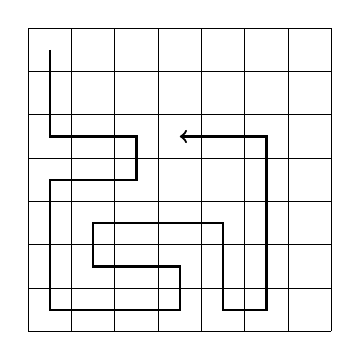
\begin{tikzpicture}[scale=.55]
  \begin{scope}
    \draw (0, 0) grid (7, 7);
    \draw[thick,->] (0.5,6.5) -- (0.5,4.5) -- (2.5,4.5) --
          (2.5,3.5) -- (0.5,3.5) -- (0.5,0.5) --
          (3.5,0.5) -- (3.5,1.5) -- (1.5,1.5) --
          (1.5,2.5) -- (4.5,2.5) -- (4.5,0.5) --
          (5.5,0.5) -- (5.5,4.5) -- (3.5,4.5);
  \end{scope}
\end{tikzpicture}
\end{center}
Thus, we can terminate the search in all such cases.
After this optimization, the search will be
very efficient:

\begin{itemize}
\item
running time: 0.6 seconds
\item
recursive calls: 69 millions
\end{itemize}

~\\
Now it is a good moment to stop optimizing
the algorithm and see what we have achieved.
The running time of the original algorithm
was 483 seconds,
and now after the optimizations,
the running time is only 0.6 seconds.
Thus, the algorithm became nearly 1000 times
faster thanks to the optimizations.

This is a usual phenomenon in backtracking,
because the search tree is usually large
and even simple observations can effectively
prune the search.
Especially useful are optimizations that
occur during the first steps of the algorithm,
i.e., at the top of the search tree.

\section{Meet in the middle}

\index{meet in the middle}

\key{Meet in the middle} is a technique
where the search space is divided into
two parts of about equal size.
A separate search is performed
for both of the parts,
and finally the results of the searches are combined.

The technique can be used
if there is an efficient way to combine the
results of the searches.
In such a situation, the two searches may require less
time than one large search.
Typically, we can turn a factor of $2^n$
into a factor of $2^{n/2}$ using the meet in the
middle technique.

As an example, consider a problem where
we are given a list of $n$ numbers and
a number $x$.
Our task is to find out if it is possible
to choose some numbers from the list so that
their sum is $x$.
For example, given the list $[2,4,5,9]$ and $x=15$,
we can choose the numbers $[2,4,9]$ to get $2+4+9=15$.
However, if $x=10$,
it is not possible to form the sum.

A standard solution for the problem is to
go through all subsets of the elements and
check if the sum of any of the subsets is $x$.
The running time of such a solution is $O(2^n)$,
because there are $2^n$ subsets.
However, using the meet in the middle technique,
we can achieve a more efficient $O(2^{n/2})$ time solution.
Note that $O(2^n)$ and $O(2^{n/2})$ are different
complexities because $2^{n/2}$ equals $\sqrt{2^n}$.

The idea is to divide the list into
two lists $A$ and $B$ such that both
lists contain about half of the numbers.
The first search generates all subsets
of the numbers in $A$ and stores their sums
to a list $S_A$.
Correspondingly, the second search creates
a list $S_B$ from $B$.
After this, it suffices to check if it is possible
to choose one element from $S_A$ and another
element from $S_B$ so that their sum is $x$.
This is possible exactly when there is a way to
form the sum $x$ using the numbers in the original list.

For example, suppose that the list is $[2,4,5,9]$ and $x=15$.
First, we divide the list into $A=[2,4]$ and $B=[5,9]$.
After this, we create lists
$S_A=[0,2,4,6]$ and $S_B=[0,5,9,14]$.
In this case, the sum $x=15$ is possible to form,
because we can choose the number $6$ from $S_A$
and the number $9$ from $S_B$,
which corresponds to the solution $[2,4,9]$.

The time complexity of the algorithm is $O(2^{n/2})$,
because both lists $A$ and $B$ contain $n/2$ numbers
and it takes $O(2^{n/2})$ time to calculate the sums of
their subsets to lists $S_A$ and $S_B$.
After this, it is possible to check in 
$O(2^{n/2})$ time if the sum $x$ can be formed
using the numbers in $S_A$ and $S_B$.